\documentclass[12pt,fleqn]{article}
%\usepackage {psfig,epsfig} % para incluir figuras em PostScript
\usepackage{amsfonts,amsthm,amsopn,amssymb,latexsym}
\usepackage{graphicx}
\usepackage[T1]{fontenc}
\usepackage[brazil]{babel}
\usepackage{geometry}
\usepackage[utf8]{inputenc}
\usepackage[intlimits]{amsmath}
\usepackage{listingsutf8}
\usepackage{float}
\lstdefinestyle{MatlabCustom}{
	language=Matlab,
	tabsize=4,
	showspaces=false,
	showstringspaces=false
}
\lstset{language=Matlab}
\lstset{inputencoding=utf8}
\lstset{basicstyle=\scriptsize,style=MatlabCustom}
\lstset{literate=%
{ó}{{\'{o}}}1
{å}{{\aa}}1
{Å}{{\AA}}1
{ç}{{\c{c}}}1
{ã}{{\~a}}1
}
\graphicspath{{./images/}}
%alguns macros
\newcommand{\R}{\ensuremath{\mathbb{R}}}
\newcommand{\Rn}{{\ensuremath{\mathbb{R}}}^{n}}
\newcommand{\Rm}{{\ensuremath{\mathbb{R}}}^{m}}
\newcommand{\Rmn}{{\ensuremath{\mathbb{R}}}^{{m}\times{n}}}
\newcommand{\contcaption}[1]{\vspace*{-0.6\baselineskip}\begin{center}#1\end{center}\vspace*{-0.6\baselineskip}}
%=======================================================================
\usepackage{a4}                       % tamanho da página
\setlength{\textwidth}{16.0cm}        % largura do texto
\setlength{\textheight}{9.0in}        % tamanho do texto (sem head, etc)
\renewcommand{\baselinestretch}{1.15} % espaçamento entre linhas
\addtolength{\topmargin}{-1cm}        % espaço entre o head e a margem
\setlength{\oddsidemargin}{-0.1cm}    % espaço entre o texto e a margem

% Ser indulgente no preenchimento das linhas
\sloppy

\begin{document}

\pagestyle {empty}

\vspace*{-2cm}
{\bf
\begin{center}
{\large
\hspace*{0cm}Universidade de São Paulo} \\
\hspace*{0cm}Escola Politécnica \\
\hspace*{0cm}Curso de Engenharia de Computação  \\
\end{center}}
\centerline{
\includegraphics[scale=0.8]{logo-poli}}
\vspace{.5cm}
\noindent
\begin{center}
{\Large \bf Condução de calor em placa plana com fontes e sorvedouros} \\[2cm]
{\Large Tiago Koji Castro Shibata (8988730), tiago.shibata@usp.br}\\[6mm]
{\Large Deborah Hidemi Kamiguchi Watanabe (4430967), deborah.watanabe@usp.br}\\[6mm]
\vspace{.5cm}
\end{center}

{\raggedleft
\begin{minipage}[t]{8.0cm}
\setlength{\baselineskip}{0.25in}
RELATÓRIO apresentado ao Professor Alexandre Roma do MAP/IME-USP
como atividade da disciplina MAP3122 - Métodos Numéricos.
\end{minipage}\\[2cm]}

\vspace{1cm}
{\center São Paulo - SP \\[3mm]
31/03/2016 \\}

\newpage


\pagestyle {empty}
\abstract{A geração de calor está presente no dia a dia de todos os seres. Desde as perdas de energias ocorrentes na mais simples das reações biológicas, o calor muitas vezes representa a energia desperdiçada, o movimento caótico de moléculas que se dispersam do fenômeno sendo realizado.

Na engenharia, a geração de calor e principalmente o aumento de temperatura têm grandes consequências, podendo criar um ambiente desagradável em uma construção mal planejada, queimar um motor ou causar danos em equipamentos. Em eletrônica, o aumento de temperatura leva circuitos a queimarem ou desligarem-se se possuírem proteção contra sobretemperatura. Neste trabalho, focamos em um modelo simples de condução de calor, em uma placa plana. A placa possuirá fontes e sorvedouros, simulando a ação de uma placa eletrônica metálica contendo componentes integrados. Algumas regiões (com componentes) serão tradadas como fontes de calor, e a placa como um todo terá uma pequena perda de calor (representando a troca de calor com o ar).

Nesse trabalho, desejamos simular a condução de calor em uma barra ou placa a partir da equação de difusão de calor, aplicando métodos numéricos em soluções computacionais. Obteremos mapas de temperatura e fluxo de calor para diferentes condições e configurações. Apresentando a temperatura próxima aos componentes, podemos simular a temperatura na qual a placa final operará e tentar melhorar a disposição dos mesmos.}

\newpage

\tableofcontents

% Numeração em romanos para páginas iniciais (sumários, listas, etc)
%\pagenumbering {roman}
\pagestyle {plain}

\setcounter{page}{0} \pagenumbering{arabic}

\setlength{\parindent}{0in}  %espaco entre paragrafo e margem
% Espaçamento entre parágrafos
\parskip 5pt
\newpage
\section{Introdução}

%comando cria itens
\begin{itemize}
	\item introduzir o problema a ser estudado
	\item apresentar trabalhos relacionados
	\item apresentar motivação
	\item apresentar objetivos
	\item Último parágrafo deve conter a organização do documento
\end{itemize}

\section{Modelo}
Em nosso modelo, a placa plana será discretizada em múltiplos quadrados de dimensão pequena. Cada pequeno quadrado será a menor subdivisão da placa que trataremos e possuirá uma temperatura homogênea. Nesse trabalho, os elementos serão sempre uniformes, bidimensionais e retangulares.

As condições iniciais serão tomadas como temperatura homogênea em toda a placa (placa desligada e equilibrada). O calor gerado pelos componentes será tomado de seus datasheets e seu número e posições será configurável. Utiliza-se o modelo de placa bidimensional, homogênea e isotrópica, ou seja, suas propriedades não se alteram em diferentes direções ou posições e a condução térmica é constante em toda a sua extensão. Parâmetros do material necessários para o modelo são $k$ (condutividade térmica), $\rho$ (massa específica) e $c_p$ (calor específico).

Duas propriedades são de interesse nesse estudo: o fluxo de calor, que indica a passagem de energia térmica, é proporcional ao oposto do gradiente da temperatura (os operandos de u(x, y, t) foram omitidos por simplicidade) \cite{ufsc_geracao_de_calor}:

\[q = -k A \frac{\partial u}{\partial x}\]
Onde $u(x, t)$ é a temperatura em x no momento t e $A$ a área de contato.

Observe que o modelo físico de fluxo de calor indica que ele flui do local mais quente para o menos quente (gradiente negativo). Além disso, e mais importante, é a temperatura nos pontos da barra. A equação de difusão de calor é:

\[\frac{\partial u}{\partial t} = \alpha \frac{\partial^2 u}{\partial x^2} + w(x)\]

Sendo $\alpha$ o coeficiente de difusão térmica. Para materiais homogêneos e isotrópicos, $\alpha$ é constante e vale:

\[\alpha = \frac{k}{\rho c_p}\]

Foi adotado como tempo inicial o instante 0 ($t_0 = 0$).

\section{Metodologia de desenvolvimento}
O desenvolvimento foi gradual, com testes de cada parte do programa. Os diferentes métodos implementados passaram por testes unitários, onde eram comparados com implementações do sistema (implementações fornecidas pelo ambiente MATLAB/Octave). Após confirmar o funcionamento das partes, passamos a montar o programa principal. Os programas de teste chamam a implementação do trabalho e do sistema e calculam a soma de erros absolutos, mostrando-o na tela. Por exemplo, para a função de cálculo de gradiente, temos test\_grad.m (apenas partes relevantes mostradas aqui):

\lstinputlisting{test_grad_simplified.m}

Que resulta em valores da ordem de $10^{-16}$, atribuídos a arredondamento numérico.

\section{Modelagem matemática}
Em  nosso  modelo,  a  placa  plana  será  discretizada  em  múltiplos  quadrados  de dimensão pequena. Cada pequeno quadrado será a menor subdivisão da placa que trataremos e possuirá uma temperatura homogênea.

As condições iniciais serão tomadas como temperatura homogênea em toda a placa (placa desligada e equilibrada). O calor gerado pelos componentes será tomado de seus datasheets e seu número e posições será configurável. Utiliza­se o modelo de placa  bidimensional,  homogênea  e  isotrópica,  ou  seja,  suas  propriedades não  se alteram em diferentes direções ou posições e a  condução térmica é constante em toda a sua extensão. 
 
O  fluxo  de  energia  térmica,  que indica locais  com grande  variação (gradiente) de temperatura, é proporcional ao inverso do gradiente da temperatura (os operandos de u(x, y, t) foram omitidos por simplicidade)

\section{Métodos numéricos}
Mostraremos métodos aplicados para discretizar e aproximar numericamente o problema.

REESCREVER COMO del(U)/del(x)

O espaço considerado é discreto (possuimos valores da função em estudo apenas em alguns pontos) e precisamos de um método de aproximar a derivada dessa função. Podemos fazê-lo calculando os primeiros termos da série de Taylor em torno de um ponto. Suponhamos que, para os pontos $x$ e $x + \Delta x$, de temperatura $u$ conhecida, desejamos aproximar a derivada no intermédio ($u'(x + \frac{\Delta x}{2})$). Sabemos que a temperatura é contínua e infinitamente derivável. Temos, por expansão em série de Taylor com resto de Lagrange em torno de $x + \frac{\Delta x}{2}$:
\begin{equation}
\label{expansao_taylor_derivada}
\begin{array}{rcl}
	u(x) & = & u(x + \frac{\Delta x}{2}) - u'(x + \frac{\Delta x}{2}) \frac{\Delta x}{2} + u''(\xi_1) \frac{(\frac{\Delta x}{2}) ^ 2}{2} \\ \\
	u(x + \Delta x) & = & u(x + \frac{\Delta x}{2}) + u'(x + \frac{\Delta x}{2}) \frac{\Delta x}{2} + u''(\xi_2) \frac{(\frac{\Delta x}{2}) ^ 2}{2}
\end{array}
\end{equation}

Onde $\xi_1$ é algum ponto entre $x$ e $x + \frac{\Delta x}{2}$ e $\xi_2$ entre $x + \frac{\Delta x}{2}$ e $x + \Delta x$. Subtraíndo a segunda equação da primeira, temos:
\[u(x + \Delta x) - u(x) = u'(x + \frac{\Delta x}{2}) \Delta x + u''(\xi_1) \frac{\Delta x ^ 2}{8} - u''(\xi_2) \frac{\Delta x ^ 2}{8}\]

Ou seja:
\[u'(x + \frac{\Delta x}{2}) = \frac{u(x + \Delta x) - u(x)}{\Delta x} + u''(\xi_2) \frac{\Delta x}{8} - u''(\xi_1) \frac{\Delta x}{8}\]

Portanto podemos aproximar a derivada em um ponto médio a dois de valores conhecidos como $\frac{u(x + \Delta x) - u(x)}{\Delta x}$ com erro $u''(\xi_2) \frac{\Delta x}{8} - u''(\xi_1) \frac{\Delta x}{8}$. Majorando o erro, temos:

\[|erro| \leq |\max_{x \leq \xi_{max} \leq x + \Delta x} u''(\xi_{max}) \frac{\Delta x}{8} - \min_{x \leq \xi_{min} \leq x + \Delta x} u''(\xi_{min}) \frac{\Delta x}{8}|\]

Com $\xi_{max}$ e $\xi_{min}$ como valores onde $u''$ é máximo e mínimo entre $x$ e $x + \Delta x$. Para $\frac{\Delta x}{8}$ pequeno, a aproximação será boa. Além disso, o problema de condução de calor tende a $u'' = 0$ (temperatura crescendo/decrescendo uniformemente), portanto esperamos que $u''$ seja pequeno conforme a simulação avança.

De posse de aproximações boas para $u'(x - \frac{\Delta x}{2})$ e $u'(x + \frac{\Delta x}{2})$, podemos calcular a derivada nos pontos de estudo ($u'(x)$) pela média entre as derivadas ($\frac{u'(x - \frac{\Delta x}{2}) + u'(x + \frac{\Delta x}{2})}{2}$). Aplicando expansão em série de Taylor $u'$ em torno de $x$, temos um sistema semelhante a \ref{expansao_taylor_derivada}:

\begin{equation}
\label{expansao_taylor_derivada_central}
\begin{array}{rcl}
	u'(x + \frac{\Delta x}{2}) & = & u'(x) + u''(x) \frac{\Delta x}{2} + u'''(\xi_1) \frac{(\frac{\Delta x}{2}) ^ 2}{2} \\ \\
	u'(x - \frac{\Delta x}{2}) & = & u'(x) - u''(x) \frac{\Delta x}{2} + u'''(\xi_2) \frac{(\frac{\Delta x}{2}) ^ 2}{2}
\end{array}
\end{equation}

Somando as equações, temos:

\[
u'(x + \frac{\Delta x}{2}) + u'(x - \frac{\Delta x}{2}) = 2u'(x) + u'''(\xi_1) \frac{\Delta x}{8} + u'''(\xi_2) \frac{\Delta x}{8}
\]

Ou seja, $u'(x) = \frac{u'(x + \frac{\Delta x}{2}) + u'(x - \frac{\Delta x}{2})}{2}$ com $|erro| \leq \max_{x - \frac{\Delta x}{2} \leq \xi_{max} \leq x - \frac{\Delta x}{2}} 2u'''(\xi_{max}) \frac{\Delta x}{8}$. Para $\Delta x$ suficientemente pequeno, calcular $u'$ como a média das derivadas laterais é uma boa aproximação.

Na figura \ref{fig:derivative_aprox} é mostrado um gráfico ilustrando a aproximação da derivada conhecendo alguns pontos de uma função. São desenhados alguns pontos de $x^2 + 1.4$. Para cada par de pontos consecutivos, aproximamos a derivada no centro do intervalo. Para análise numérica, nos interessa aproximar a derivada nos pontos dados e não nos intermediários, e a aproximamos calculando a média entre intermediários consecutivos.

\begin{figure}[H]
	\centering
		\includegraphics[height=12cm]{derivative_aprox}
		\caption{Aproximação da derivada}
		\label{fig:derivative_aprox}
\end{figure}

Comparamos os resultados com a função de aproximação da derivada do ambiente de desenvolvimento em vetores aleatórios e obtivemos erro negligível (soma de erros absolutos da ordem de $10^{-16}$ em matriz 8x8 gerada pela função $rand()$, que retorna números de 0 a 1).

Para formular a aproximação da segunda derivada, também fizemos expansão em polinômio de Taylor com resto de Lagrange:

\begin{array}{rcl}
	u(x + \Delta x, t) & = & u(x, t) + \frac{\partial u}{\partial x}(x, t) \Delta x + \frac{\partial^2 u}{\partial x^2}(x, t) \frac{\Delta x ^ 2}{2} + \frac{\partial^3 u}{\partial x^3}(x, t) \frac{\Delta x ^ 3}{6} + \frac{\partial^4 u}{\partial x^4}(\xi_1, t) \frac{\Delta x ^ 4}{24} \\ \\
	u(x - \Delta x, t) & = & u(x, t) - \frac{\partial u}{\partial x}(x, t) \Delta x + \frac{\partial^2 u}{\partial x^2}(x, t) \frac{\Delta x ^ 2}{2} - \frac{\partial^3 u}{\partial x^3}(x, t) \frac{\Delta x ^ 3}{6} + \frac{\partial^4 u}{\partial x^4}(\xi_2, t) \frac{\Delta x ^ 4}{24}
\end{array}

De maneira similar a feira para a primeira derivada, somando as equações, rearranjando os termos e majorando $\xi_1$ e $\xi_2$, obtemos:

\[|erro| \leq \max_{x \leq \xi_{max} \leq x + \Delta x} u''(\xi_{max}) \frac{\Delta x}{8} - \min_{x \leq \xi_{min} \leq x + \Delta x} u''(\xi_{min}) \frac{\Delta x}{8}\]

\begin{equation}
	\frac{\partial^2 u}{\partial x^2}(x, t) = \frac{u(x + \Delta x, t) + u(x - \Delta x, t) - 2 u(x, t)}{\Delta x^2} - \frac{\Delta x^2}{12} \frac{\partial^2 u}{\partial x^2} (\xi, t), \xi \in [x - \Delta x, x + \Delta x]
\end{equation}

Portanto, o erro

\section{Exemplos de Equações}
Nesta seção serão apresentados diferentes exemplos de equações.

\subsection{Equações simples}

\textbf{Sem numeração}
\[\sum_{i=1}^{100}\frac{2^{i-1}}{4}\]

\textbf{Com numeração}
\begin{equation}
	\int_{0}^{100}\sqrt[4]{\frac{2n}{7}}
\end{equation}

\begin{equation}
M^{-1}(AD^{-1}A^T)M^{-T}\bar{y} = M^{-1}(AD^{-1}(r_d -X^{-1}r_a) + r_p),
\end{equation}


\subsection{Equações com mais de uma linha}
\begin{eqnarray}
\label{pp}
\min & c^Tx \\ \nonumber
\mbox{s.a.} & Ax=b \\ \nonumber
            & x \geq 0, \nonumber
\end{eqnarray}
onde $A \in \Rmn$, $b \in \Rm$ and $c \in \Rn$.
Referenciando a equação ~(\ref{pp})

\subsection{Sistema linear}

\begin{equation}
 \left[
\begin{array}{ccc}
 A & 0   & 0 \\
 0 & A^T & I\\
 Z & 0   & X
\end{array} \right]
\left[
\begin{array}{c}
 x \\
 y \\
 z \\
\end{array}
\right]
=
\left[
\begin{array}{c}
 1 \\
 2 \\
 3
\end{array}
\right]
\label{eqpc0}
\end{equation}

\[
d_i=\left \{
\begin{array}{cc}
1 & \mbox{se } i=0 \\
2 & \mbox{caso contrário}\\
\end{array}
\right \}
\]

%inicia uma nova p�gina
\clearpage

\section{Tabelas}
\label{sec:tab}


\subsection{Tabela Simples}
\begin{table}[htb]
\begin{center}
		\begin{tabular}{|c|c|c|}\hline
		12  & 13 & 14 \\\hline
		15  & 16 & 17 \\\hline
		\end{tabular}
\label{tab:Tabela1}
\caption{Título da tabela}
\end{center}
\end{table}


\subsection{Tabela mais elaborada}
\begin{table}[htb]
\begin{center}
\begin{tabular}{|l|r|c|r|r|} \hline
            & \multicolumn{2}{|c|}{{CCF preconditioner}} & \multicolumn{2}{|c|}{{Number of nonzeros}} \\ \cline{2-5}
{Problem}   & \multicolumn{1}{|c|}{$\eta$}  & \multicolumn{1}{|c|}{$ \frac{n(AD^{-1}A^T)}{nrow}$} & \multicolumn{1}{|c|}{FCC} & \multicolumn{1}{|c|}{Cholesky}  \\ \hline \hline
ELS-19    &  -11 & 31 &  87750  & 3763686  \\\hline
SCR20     &  -12 & 31 &  103179 & 2591752  \\\hline
NUG15     &  -12 & 32 &  54786  & 6350444 \\\hline
PDS-20    &   15 & 5  &  625519 & 7123636\\\hline
\end{tabular}
\caption{Título da Tabela.}
\label{tabn}
\end{center}
\end{table}

Referenciando a tabela~\ref{tabn}.

\section{Edição}

Comando para preservar a formatação do texto.
\begin{verbatim}
#include <iostream>         // < > is used for standard libraries.
void main(void)             // ''main'' method always called first.
{
 cout << ''This is a message.'';
                            // Send to output stream.
}
\end{verbatim}

\section{Inserir figuras}

\begin{figure}[htb]
	\centering
		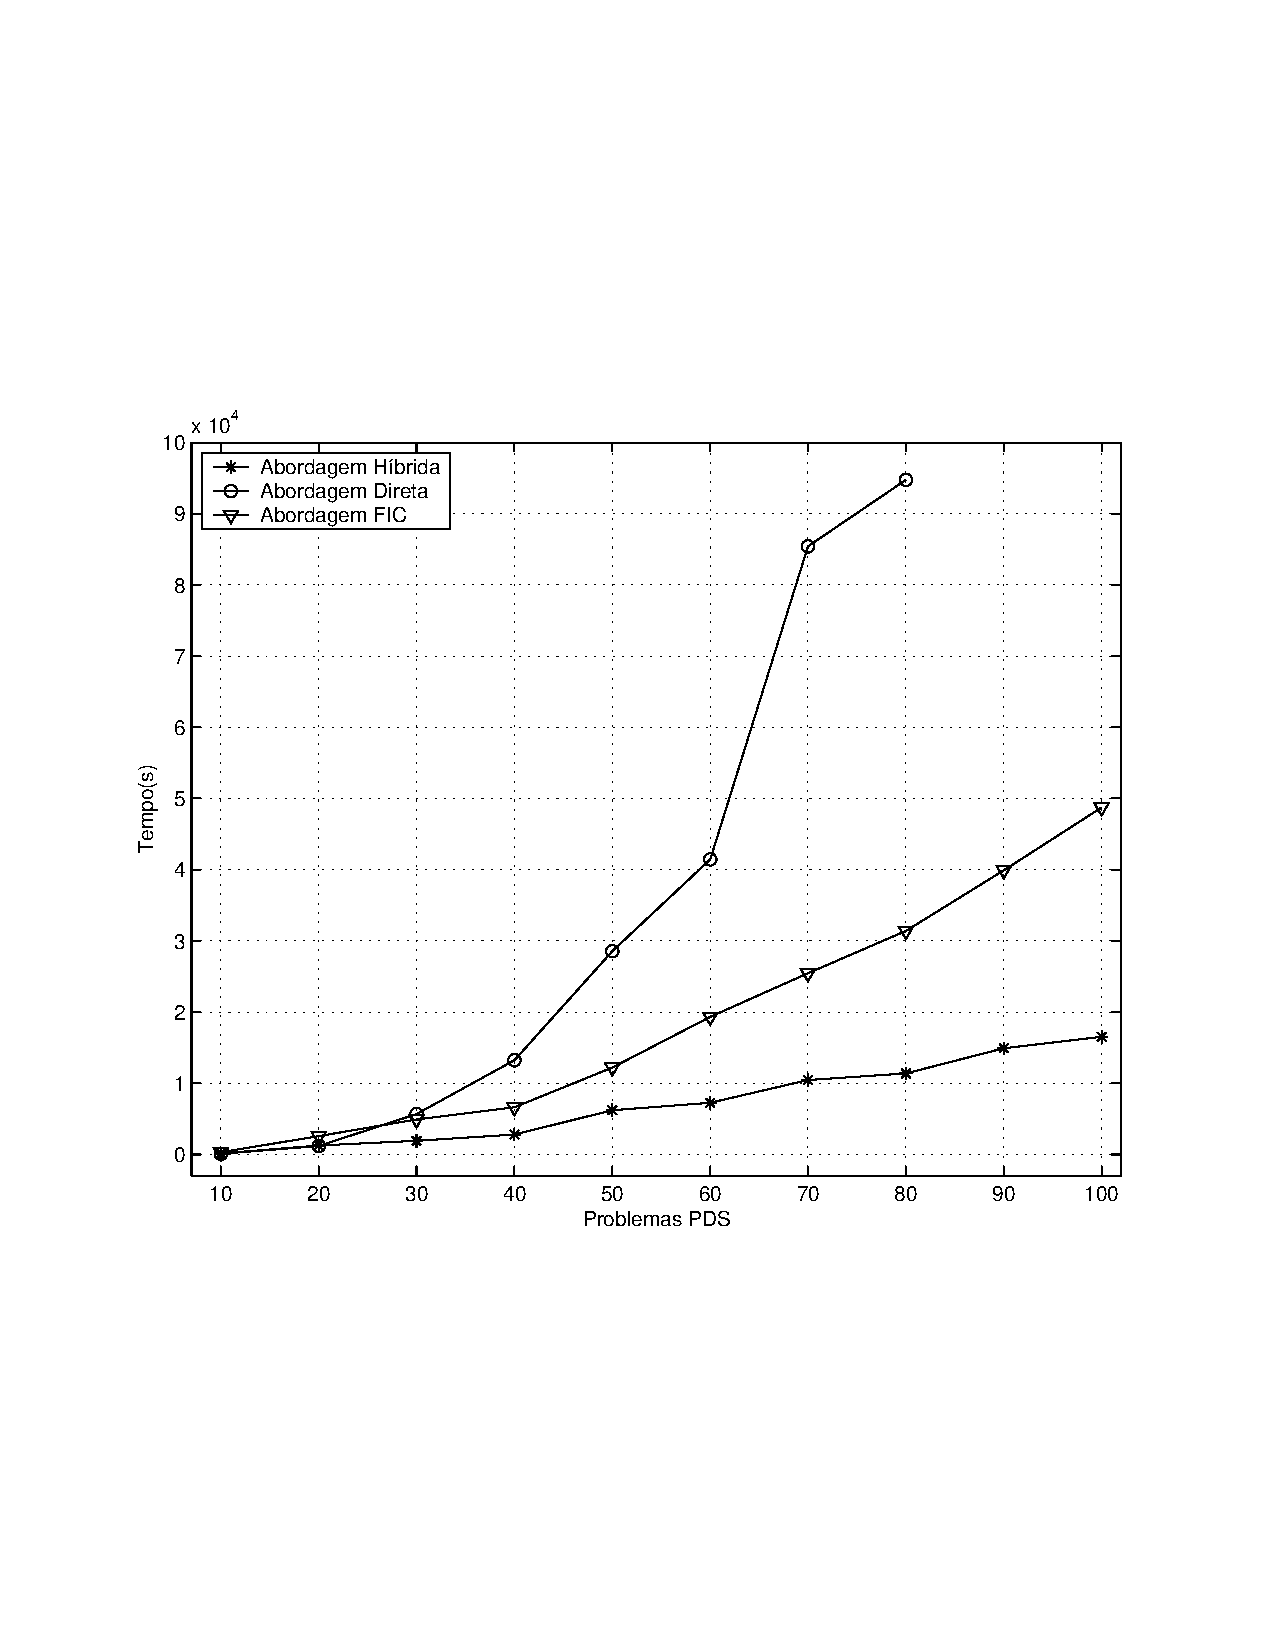
\includegraphics[height=14cm]{figura}
	\label{fig:pdsmodel}
\end{figure}

%\clearpage %come�a nova p�gina

Para citar referências bibliográficas~\cite{Adler89}, \cite{Carmo05}.

\section{Conclusões}
Apresentar as conclusões finais.

\vspace{5mm}
{\bf{Agradecimentos}} Agradecimentos aos colaboradores, professores que eventualmente procuraram para ajudar em
algum aspecto do modelo, colega que ajudou a compor alguma parte do trabalho e assim por diante.

\bibliographystyle{plain}
\bibliography{bibliografia}

% aqui, viriam os ap�ndices se viessem (fica como atividade descobrir como introduz�-los

\end{document} %finaliza o documento
